A Recurrent neural network(RNN), is a neural network model with principle of saving the output, feeding this output as input to the same model. RNNs works with sequences of arbitrary lengths. Sequences are a sets of data having a defined order to it. In our case the sequential data we are working with are the amino acid sequences. RNNs are very good at next token predictions in data.

\noindent
Next token prediction, means predicting the next element in an sequence, given the previous data points have been analyzed.

\begin{figure}[!ht]
  \centering
  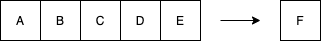
\includegraphics[scale=0.4]{latex/IMGs/AlphabetPred.png}
  \caption{Simple example of how an RNN can predict the next element in the alphabet}\label{Baseline:before}
\end{figure}

\noindent
As for a feed forward neural network, a RNN also has an input layer, hidden layer, and a output layer. Essientially,